% !TEX root = Bachelorarbeit.tex
\subsection{The seL4 Microkernel}\label{sec:seL4}
	The seL4 \cite{Manual} ist a small operation system kernel. It's based on the in the L4 microkernel developed in the 1990s and provieds a minimal number of services to applications, such as abstractions for virutal address spaces, threads, inter process comunication (IPC). \\
	Each abstraction ist implemented by a kernel object with methodes dependent on the abstraction it supplies. The objects can be named and accessed by capablities which are also stored in kernel objects called \textit{CNodes}. \\
	Each capability contains a target object and potentially several access rights. The access rights can be \texttt{Read, Write, Grant} and \texttt{Create}. By invoking a capability that points to the kernel object  with a corresponding method name, applications can invoke system calls. As arguments these system calls can have data or other capabilities. 

\subsubsection{System Calls}
Kernel provided system calls:
\begin{itemize}
\item \texttt{send()}: The system call argument ist delivered to the target object and the application is allowed to continue. If the target is not able to receive and/or process the arguments immediately, the sending application will be blocked until the arguments can be delivered.

\item \texttt{NBSend()}: Like \texttt{send()}. Exception: If the message is not deliverable it's silently droped.
\item \texttt{Call()}: Like \texttt{send()} but the application is blocked until the object provides a response, or the receiving application replies. \\
If the argument is delivered to an application via Endpoint the receiver needs the right to respond to the sender. So in this case an additional capability is added to the arguments. 
\item \texttt{Wait()}: If the target object is not ready \texttt{Wait()} is used by an application to block until the object is ready. 
\item \texttt{Reply()}: Used to respond to a \texttt{Call()}, using the capability generated by the \texttt{Call()} operation.
\item \texttt{ReplyWait()}: As a combination of \texttt{Reply()} and \texttt{Wait()} it is efficent for the common case that replying to a request and waiting for the next can be performed in a single system call. 
\end{itemize}
	
\subsubsection{Kernel Objects}\label{sec:KernelObjects}
The kernel implements several objects to allocate the system operations \cite{Manual}.
\begin{itemize}
\item \textbf{CNodes} \\
The capabilities to invoke system calls are stored in \textbf{\textit{CNodes}}. When created they get a fixed numer of slots that can be empty or contain a capability. 
The kernel conducts a \textbf{Capability Derivation Tree} (CDT) to keep records about the created capabilities and their associations. This is required for the revoke operation. \\ 
They have the following operations:
\begin{itemize}
\item \texttt{Mint()} \\
creates a copy of an existing capability. The new capability is placed in a specified CNode slot and may have less rights than the parent capability. In the CDT the capability is placed as child of the original one. 
\item \texttt{Copy()} \\
is similar to the Mint operation. But the new capability has the same rights as the original one and in the CDT it's represented as a sibling of it. 
\item \texttt{Move()} \\
can maneuver a capability between two specified slots. 
\item \texttt{Mutate()} \\
moves the capability similar to \texttt{Move()} and is able to reduce its rights as it is done in \texttt{Mint()} without an orignal copy remaining.
\item \texttt{Rotate()} \\
moves two capabilities between three slots. Replaces two \texttt{Move()} operations. 
\item \texttt{Delete()} \\
can remove a capability from a specified slot.
\item \texttt{Revoke()} \\
is used to remove a complete part of the CDT. From a defined capability on, all children from the capability in the CDT are removed with \texttt{Delete()}. 
\item \texttt{Recycle()} \\
revokes all outstanding capabilities and reconfigures the object to its initial state. So the object can be reused in for another purpose.
\end{itemize}

\item \textbf{IPC Endpoints} \\
Endpoints are used for the \textit{interprocess communication} between threads. They can be devided into \textbf{synchronous (EP)} and \textbf{asynchronous (AEP)} endpoints. 
Threads in the seL4 kernel are grouped into security domains. Interprocess communication between different domains is only realised via AEPs. Generally capabilities to endpoints can be restricted to be read - or write - only. 
\item \textbf{TCP} \\
A thread of execution in seL4 is represented by a \textit{thread control block}. It is always associated with a CSpace (provides the capabilities required to manipulate the kernel objects) and a VSpace (provides the virtual memory environment required to contain the code and data application). \\
The TCB object has the following methods: \\
\texttt{CopyRegisters(), ReadRegisters(), WriteRegisters(), SetPriority(), \\ SetIPCBuffer(), SetSpace(), Configure(), Suspend(), Resume()}
	\begin{figure}[ht]
	\centering
		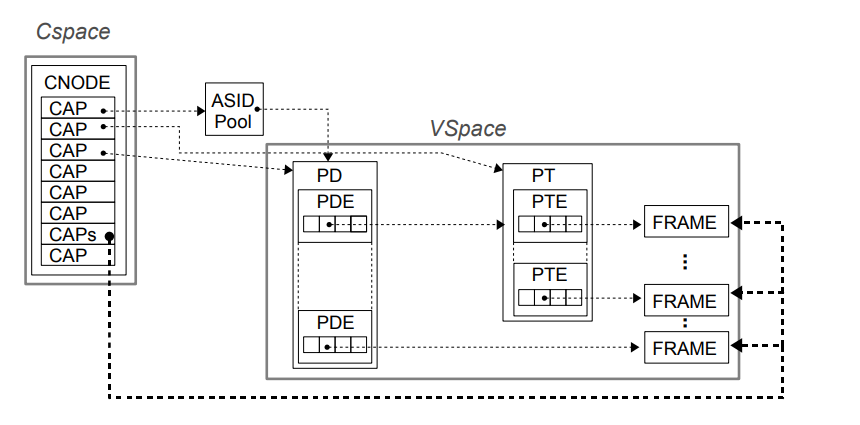
\includegraphics[width=0.7\textwidth]{./Pictures/applicationIntern.png}
	\caption[Internal representation of an application]{Internal representation of an application in seL4 \cite{sel4}}
	\label{fig:intapp}
	\end{figure}
	
\item \textbf{Virtual Memory}\\
Objects in the \textit{virtual address space} (VSpace) implement services for the management of virtual memory which largely directly correspond to those of the hardware: \\
Page Directory, Page Table, Page, ASID Control, ASID Pool \\
Figure \ref{fig:intapp} showes how they are connected.
\item \textbf{Interrupt Objects} \\
Device driver applications require \texttt{Interrupt Ojects} to be capable of receiving and acknowledging interrupts from hardware devices.
\item \textbf{Untyped Memory} \\
\texttt{Untyped memory objects (UMO)} encapsulate a fixed-sized, size-aligned, continuous region of the physical memory. Each object can be devided into a group of smaller untyped memory objects. With \texttt{Retype()} a number of new kernel objects are created. It also returns capabilities to the new objects if it succeeds. 
\end{itemize}

\subsubsection{Memory Allocation Model} 
A special characteristic of the seL4 is that the memory for kernel objects is not allocated dynamically. A goal was to isolate physical memory access between applications and to control the amount of physical memory that applications can use. \\
For this applications get fixed sized memory reagions they have to control by themselves. \\
Capabilities on Untyped Memory Objects (UMO) are needed to create new objects. So applications need the capabilities on UMOs to create new objects. After creation the objects have a fix amount of memory they can use. \\
At boot time the kernel pre-allocates all the memory required for the kernel to run. This includes the space for kernel code, data and kernel stack. The kernel then creates an \textit{Initial User Thread} with associated CSpace and VSpace and hands over the remainig memory in form of capabilities on UMOs. \\
The Initial User Thread can create smaler sized UMOs out of an UMO or \texttt{retype} it into another object type. The creator of new objects has full authority over the objects. This "full authority" depends on the object type. \\
Figure \ref{fig:systarch} shows a sample system architecture in which a resource manager running at user-level  has the authority to the remaining untyped memory after boot strapping. 
	
	\begin{figure}[ht]
	\centering
		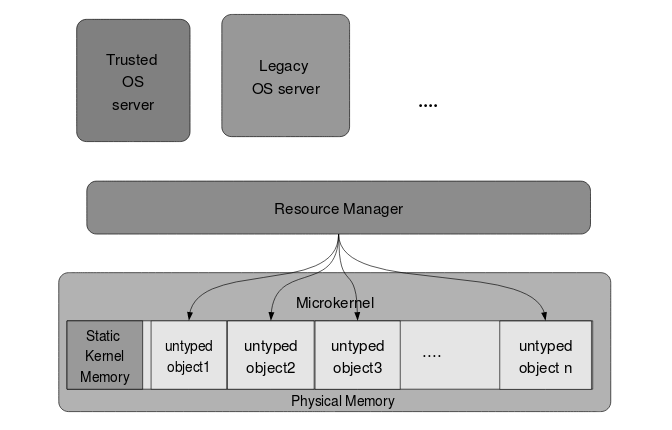
\includegraphics[width=0.6\textwidth]{./Pictures/MemoryAllocation.png}
	\caption[Sample system architecture]{Sample System Configuration \cite{TakeG}}
	\label{fig:systarch}
	\end{figure}	